\documentclass[xelatex,ja=standard,jafont=noto]{bxjsarticle}
\usepackage[utf8]{inputenc}

\usepackage{amsmath}
\usepackage{amsthm}
\usepackage{amssymb}
\usepackage{mathrsfs}
\usepackage{graphicx} 

\usepackage{tikz}
\usetikzlibrary{shapes,arrows}
\usepackage{verbatim}
\tikzstyle{block} = [draw, fill=white, rectangle, 
    minimum height=3em, minimum width=6em]
\tikzstyle{sum} = [draw, fill=white, circle, node distance=1cm]
\tikzstyle{input} = [coordinate]
\tikzstyle{output} = [coordinate]
\tikzstyle{pinstyle} = [pin edge={to-,thin,black}]



\newtheorem{theorem}{Theorem}
\newtheorem{corollary}{Corollary}
\newtheorem{lemma}{Lemma}
\newtheorem{example}{Ex\documentclass{article}
	\usepackage{CJKutf8}
	\usepackage{amsmath}
	\usepackage{amsthm}
	\usepackage{amssymb}
	ample}
\newtheorem{definition}{Definition}

\def\ds{\displaystyle}
\def\ul{\underline}
	
	\title{Report No.4	}
	\author{BQ18026,関宇 }
	\date{June 9,2020}
	
\begin{document}
		\maketitle
	
	\section{RLC回路}
		
		
\begin{equation}
\left\{
             \begin{array}{lr}
             	v_{i}(t)=Ri(t)+v_{0}(t)+L\frac{di(t)}{dt} &  \\
             v_{0}(t)=\frac{1}{C}\int_{0}^{t}i(\tau)d\tau &  
             \end{array}
\right.
\end{equation}
		
		
		まず、ラプラス変換を計算する
		
		
\begin{equation}
\left\{
             \begin{array}{lr}
             		V_{I}(s)-V_{0}(s)=RI(s)+LsI(s) \\
            V_{0}(s)=\frac{1}{Cs}I(s) &  
             \end{array}
\right.
\end{equation}

		 
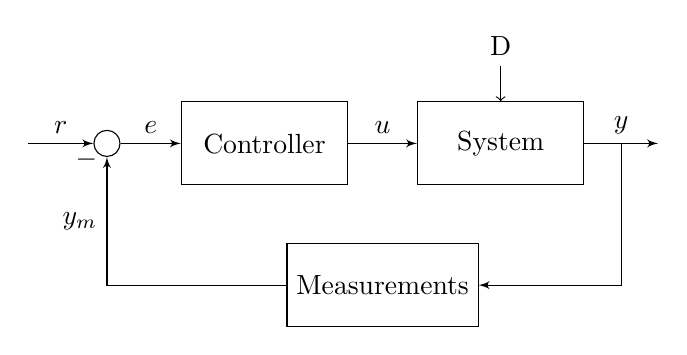
\begin{tikzpicture}[auto, node distance=2cm,>=latex']

    \node [input, name=input] {};
    \node [sum, right of=input] (sum) {};
    \node [block, right of=sum] (controller) {Controller};
    \node [block, right of=controller, pin={[pinstyle]above:D},
            node distance=3cm] (system) {System};

    \draw [->] (controller) -- node[name=u] {$u$} (system);
    \node [output, right of=system] (output) {};
    \node [block, below of=u] (measurements) {Measurements};

    \draw [draw,->] (input) -- node {$r$} (sum);
    \draw [->] (sum) -- node {$e$} (controller);
    \draw [->] (system) -- node [name=y] {$y$}(output);
    \draw [->] (y) |- (measurements);
    \draw [->] (measurements) -| node[pos=0.99] {$-$} 
        node [near end] {$y_m$} (sum);
\end{tikzpicture}


		 
		  \begin{equation}
		 G_{4}(s)=\frac{s+2}{s^{3}+s^{2}+s+1}
		 \end{equation}
		 
		 \[  G_{4}(s)=\frac{s+2}{(s+1)(s^{2}+1)}=\frac{s+2}{(s+1)(s+i)(s-i)}  \]
		 
		 虚軸上に極が持っているので、この伝達関数が不安定である。
		 
		  \begin{equation}
		 G_{5}(s)=\frac{s-1}{s^{3}+3s^{2}+s+1}
		 \end{equation}
		 ここで特性多項式から係数を抜け出して、フルビッツ行列から安定性を求める。
		  \[  a_{3}=1,a_{2}=3,a_{1}=1,a_{0}=1  \]
		  よって
		  \[ H=
		  \left|\begin{array}{cccc} 
		  3 &    1    & 0 \\ 
		  1 &    1    & 0 \\ 
		  0 &    3    & 1 
		  \end{array}\right| 
		  \]
		  
		  \[  H_{1}=3,H_{2}=2,H_{3}=2  \]
		  従って、システムが安定である
		 
		 \section{}
		 
		 \[ D(s)=s^{3}+a_{2}s^{2}+a_{1}s+a_{0}  \]
		 まずこの多項式のフルビッツ行列を求める
		  \[ a_{3}=1,a_{2},a_{1},a_{0}  \]
		  よって
		  
		\begin{equation}
	H=
	\left|\begin{array}{cccc} 
	a_{2} &    a_{0}    & 0 \\ 
	1 &    a_{1}    & 0 \\ 
	0 &    a_{2}   & a_{0} 
	\end{array}\right| 
	    \end{equation}
	 安定性の条件より、   
	   \[  a_{2}>0,a_{2}a_{1}>a_{0},a_{0}>0,a_{1}>0  \]
	    
	    
	    \section{次の二次系の伝達関数が与えられている.}
	    
	\[  H_{1}(s)=\frac{2}{s^{2}+2s+2},H_{2}(s)=\frac{5}{s^{2}+2s+5} \]
		
	まずH1、H2の極が求める。
		 
	\[  s1=-1\pm i,s2=-1\pm 2i \]
	両方の極の実数部がともに正であるので、両方とともに安定である。しかし複数の部分が伝達関数の振動を支えられている。両方の周期を比べると
		 \[  \omega_{1}=2\pi,\omega_{2}=\pi \]
		 
		 
		よって、H2のほうが速く収束している。\\
	次に、最終値定理を使ってステップ入力の最終値を求める。
		 \begin{equation}
		 \lim_{t \to \infty} h_{1}(t) = 2, \lim_{t \to \infty} h_{2}(t) = 5
		 \end{equation}
		 
		 \newpage
		
		\section{有界な時間関数とは何か,定義を述べ,例を挙げよ.}
		ある有界の正の値Mが存在する。もしある関数の任意の値の絶対値がMより小さければ、この関数は有界である。例えばsin(t),cos(t).tはいくらになってもこの関数の絶対値が1に超えられない。逆にt=xは有界ではない。xが無限大になるとtも無限大になる。\\
		しかし、無界関数の中で、とくに微妙だと思うことがある。
		
		 \begin{equation}
		x=1+\frac{1}{2}+\frac{1}{3}+\frac{1}{4}.....
		\end{equation}
	このような関数は実は有界ではない。

\end{document}